\scanpage{93}
\mspage{14}
action on \deleted{$H_{x_i,x_0}$} the system $(\Pi_0,H_{x_i,x_0},\underbrace{\Pi_0/\Pi'_0}_{\deleted{\unsure{space|space}}})$ where we let $\Theta$ act on $\Pi_0,H_{(x_i,x_0)}$ through its action on $\mathcal C$, and on $\Pi_0/\Pi'_0$ via the action on $\Pi_0$, which descends to the quotient by the \deleted{hypothesis} \inserted{condition} \deleted{said} under consideration. The \deleted{extended} lifted action \inserted{$\unsure{\widetilde\Theta|\Theta'}$ of $\Theta$} \deleted{is} on $\widetilde{\mathcal C}$ is therefore unique. For there to exist an action of $\Theta^{*}$ on $\mathcal C'$ which is compatible with $\mathcal C'-\mathcal C$, it is necessary and sufficient that the preceding condition be satisfied, and that \uline{in addition} $\operatorname{Ob}\mathcal C'\subset\operatorname{Ob}\mathcal C$ be stable under \deleted{this} the action of $\widetilde\Theta$.

In the case where we do not assume that we \deleted{have at our disposal} \inserted{give} an $x'_0\in\operatorname{Ob}\mathcal C'$ which we require to be fixed by $\Theta$, we consider the fiber \inserted{$E_0=$} $\widetilde{\mathcal C}_{x_0}$, which is a \deleted{\unsure{a}} homogeneous $\Pi_0$-set, and we note that the ways of lifting $\Theta$ to an action \inserted{$\unsure{\overline\Theta|\widetilde\Theta}$} in $\widetilde{\mathcal C}$ correspond \deleted{\unsure{to the}} exactly to the ways of lifting $\Theta$ to an action of $\widetilde\Theta_0$ on $E_0$, \deleted{\unsure{how|suitable}} be compatible with the action on $\Pi_0$, i.e satisfying
\margin{but we still assume an $x_0$ fixed under $\Theta$}
\figure{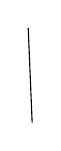
\begin{tikzpicture}\draw(0,0)--(-.05,1.2);\end{tikzpicture}}
\margin{This holds without assuming $\widetilde{\mathcal C}$ connected --- but the translation below in terms of $\Pi'_0\subset\Pi_0$ depends on the connectedness condition.\ldots Cf below the case where we have a connected full \unsure{s-grp} $\mathcal C$}
\[
\tag{46}\widetilde\Theta_0(g.x^{\deleted{\unsure{0}}\prime})\mathord{\hbox{\begin{tikzpicture}[baseline=0pt]\path[use as bounding box] (-.015,0) rectangle (.05,.28);\fill (0,.19) circle[radius=.010];\fill (.035,.26) ellipse[x radius=.010,y radius=.014];\end{tikzpicture}}}=\Theta(g)\widetilde\Theta_0(x')
\]
--- \deleted{it corresponds} \inserted{such an action} is known when we \unsure{know|know}, for \uline{one} fixed $x'_0$ of $E_0=\operatorname{Ob}\widetilde{\mathcal C}_{x_0}$, its transform under $\widetilde\Theta_0$, formula (46) giving all the others \inserted{$\widetilde\Theta_0(x')$, \deleted{since $\unsure{x'\in E_0}$} $\unsure{\mathrm{for}|\forall}\,x'\in E_0$}. In terms
\margin{92}
